\subsection{Class Diagram}

The architecture of our webapp is based on four principal items:
\begin{itemize}
    \item \textbf{Resource}: also called POJO (Plain Old Java Object) classes are the classes that deal with the object representation of data in the database using a tree hierarchy.
    \item \textbf{DAO} (Data Access Object): are the classes that communicate with the database, taking care of the queries and saving their results in the resource classes.
    \item \textbf{Servlet}: are the classes that manage the interaction with the rest APIs and hypertext.
    \item \textbf{Filter}: are the classes that protect the servlet access allowing only those who really are entitled to it to use their functionalities.
\end{itemize}

\subsection*{Resource}

In the figure \ref{fig:ResouceClassDiagram} it is possible to observe the 
architecture of the resources, all implementing the Resource interface 
and containing the \texttt{toJSON()} method. 
The main reason for which it has been utilized an interface and not an abstract 
class is because of the greater possibilities that an interface offers in 
Java. An example could be that an enumeration can implement an interface and that it cannot 
extend an abstract class: this allows us to manage the enumerations 
as resources.

It has been used the \texttt{org.json} package (also used by the tutor), because the 
use is more  immediate and requires less code overhead than the
\texttt{fasterxml.jackson} package.


\begin{figure}[H]
    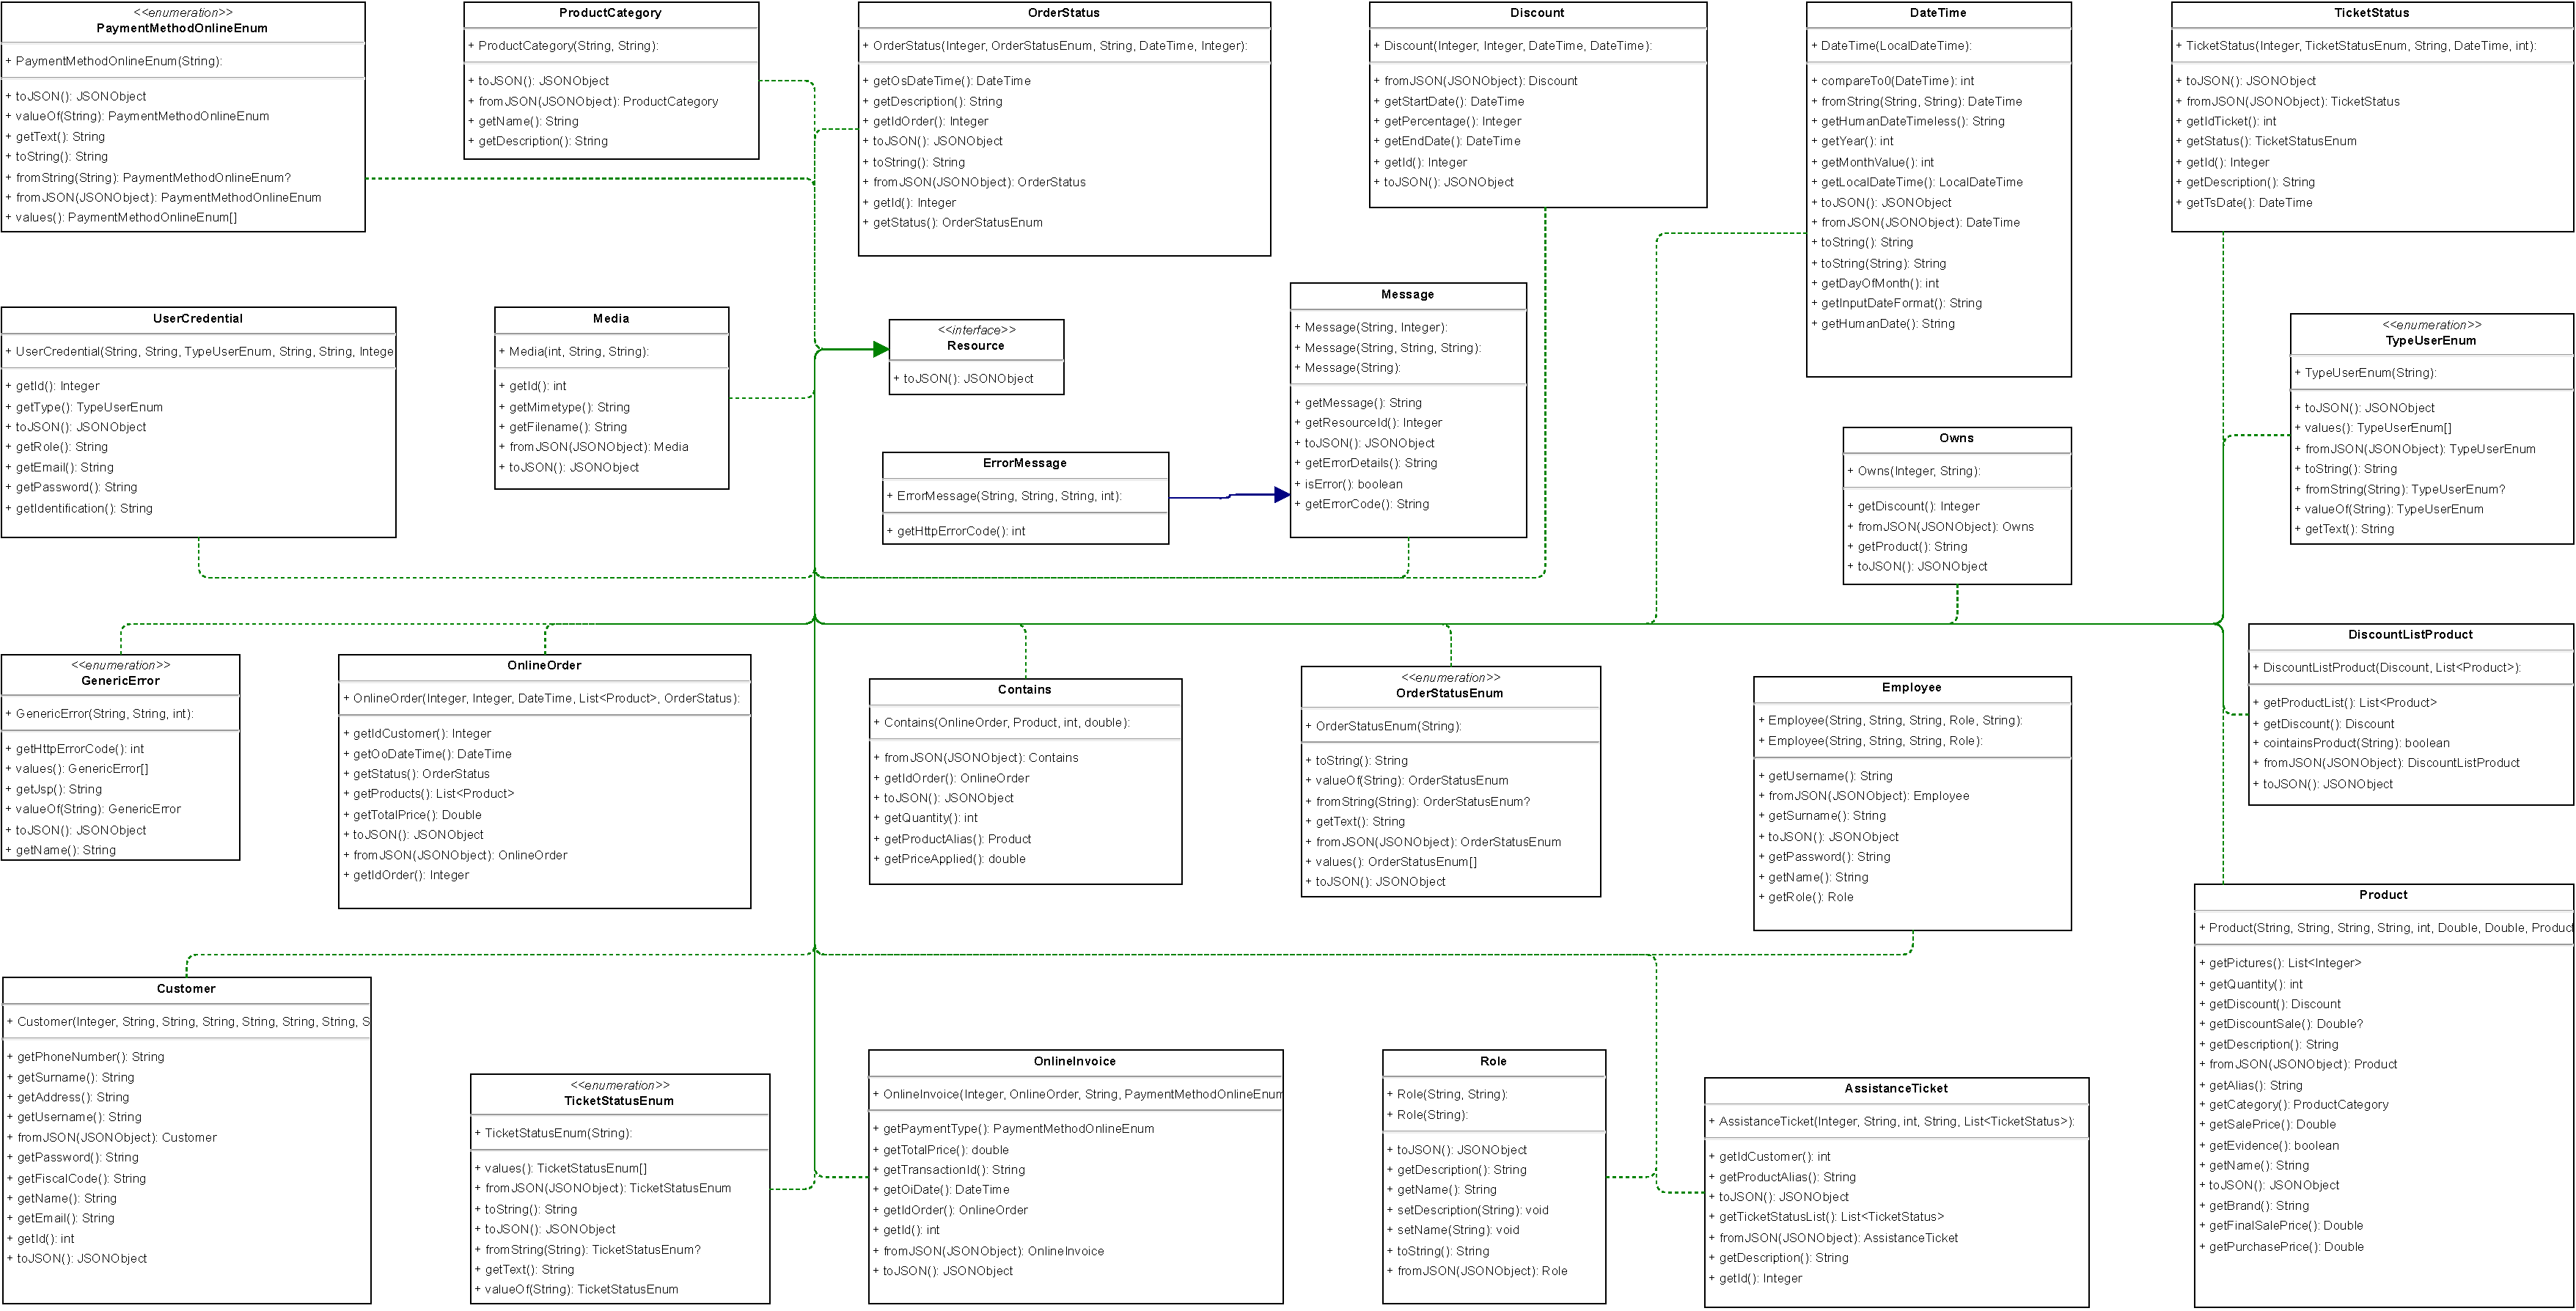
\includegraphics[width=\textwidth,height=\textheight,keepaspectratio]{Schemas/resources.drawio.pdf}
    \caption{Resource class diagram}
    \label{fig:ResouceClassDiagram}
\end{figure}

\subsection*{DAO}

Since DAOs have no inheritance (there 
is no basic DAO), we do not include the DAO schema.
Regardless, they are already divided into subpackages for the table they 
operate on, although they are an important part of the project.


\subsection*{Servlet}

In the figure \ref{fig:ServletClassDiagram} it is possible to observe the 
architecture of the servlets. 
We defined this structure in order to maintain a functional separation 
between the common web pages and the ones dedicated to the login or the database.
In particular: 
\begin{itemize}
    \item \texttt{AbstractServlet} extends \texttt{HttpServlet} and
    it contains the functions to print in output the web pages using JSON and JSP.
    \texttt{AbstractServlet} contains an abstract method that references the 
    database connection as it was needed to properly implement the header
    without breaking the Model View Controller pattern;

    \texttt{AbstractServlet} also contains functions such as 
    \texttt{writeResource, writeJsp, writeError, writeMessageOrRedirect, 
    writeJSON, writeBlob, readJSON}  and \texttt{readInputParameters}
    that allow to effectively and centrally manage all the output 
    and marginally also the input.
    In detail the functions mentioned above are responsible for: 
    \begin{itemize}
        \item \texttt{writeResource} sends the request to a JSON
        or hypertext (HTML) output based on whether or not a REST request is made. 
        Automatically provides the JSP with the session information in 
        the variable \texttt{user}.
        The first two parameters passed to the function are the HTTP request and 
        response, then we pass the JSP url followed by a boolean 
        value to indicate if we want to pass a list (false) or a single object (true) as last parameter.
        The last parameter you pass is in fact a class that implements the 
        Resource class via varargs and that supports arrays of single or multiple elements.
        \item \texttt{writeJsp} is used to print a JSP page without any resource.
        It does not print a JSON in case of REST request as there is nothing to be printed.
        \item \texttt{writeError}  is used to print an error within an
        JSON or hypertext (HTML) output based on whether or not a REST request is made. 
        \item \texttt{writeMessageOrRedirect} is used when it's necessary to realize some redirects and since this is not possible 
        using the rest API, it has been created this kind of function that is able to make 
        the redirect only if it is hypertext. In the case of a JSON output it just
        prints a message with the useful data to reach the new page.
        \item \texttt{writeJSON} is the function that prints the formatted JSON.
        \item \texttt{writeBlob} is the function that prints a blob file with 
        header and everything that the browser needs to read it.
        \item \texttt{readJSON}  is the function devoted to reading the informations 
        from the header POST in JSON format.
        \item \texttt{readInputParameters} is the function devoted to reading the 
        information from the header POST returning an array of key-value pairs.
    \end{itemize}
    \item \texttt{AbstractLoggerServlet} extends the \texttt{AbstractServlet}. It initialises Log4j
    so that each class has its own logger already initialized.
    \item \texttt{AbstractDatabaseServlet} extends \texttt{AbstractLoggerServlet}. It initialises the database.
    All servlets extend \texttt{AbstractDatabaseServlet}.
\end{itemize}    


\begin{figure}[H]
    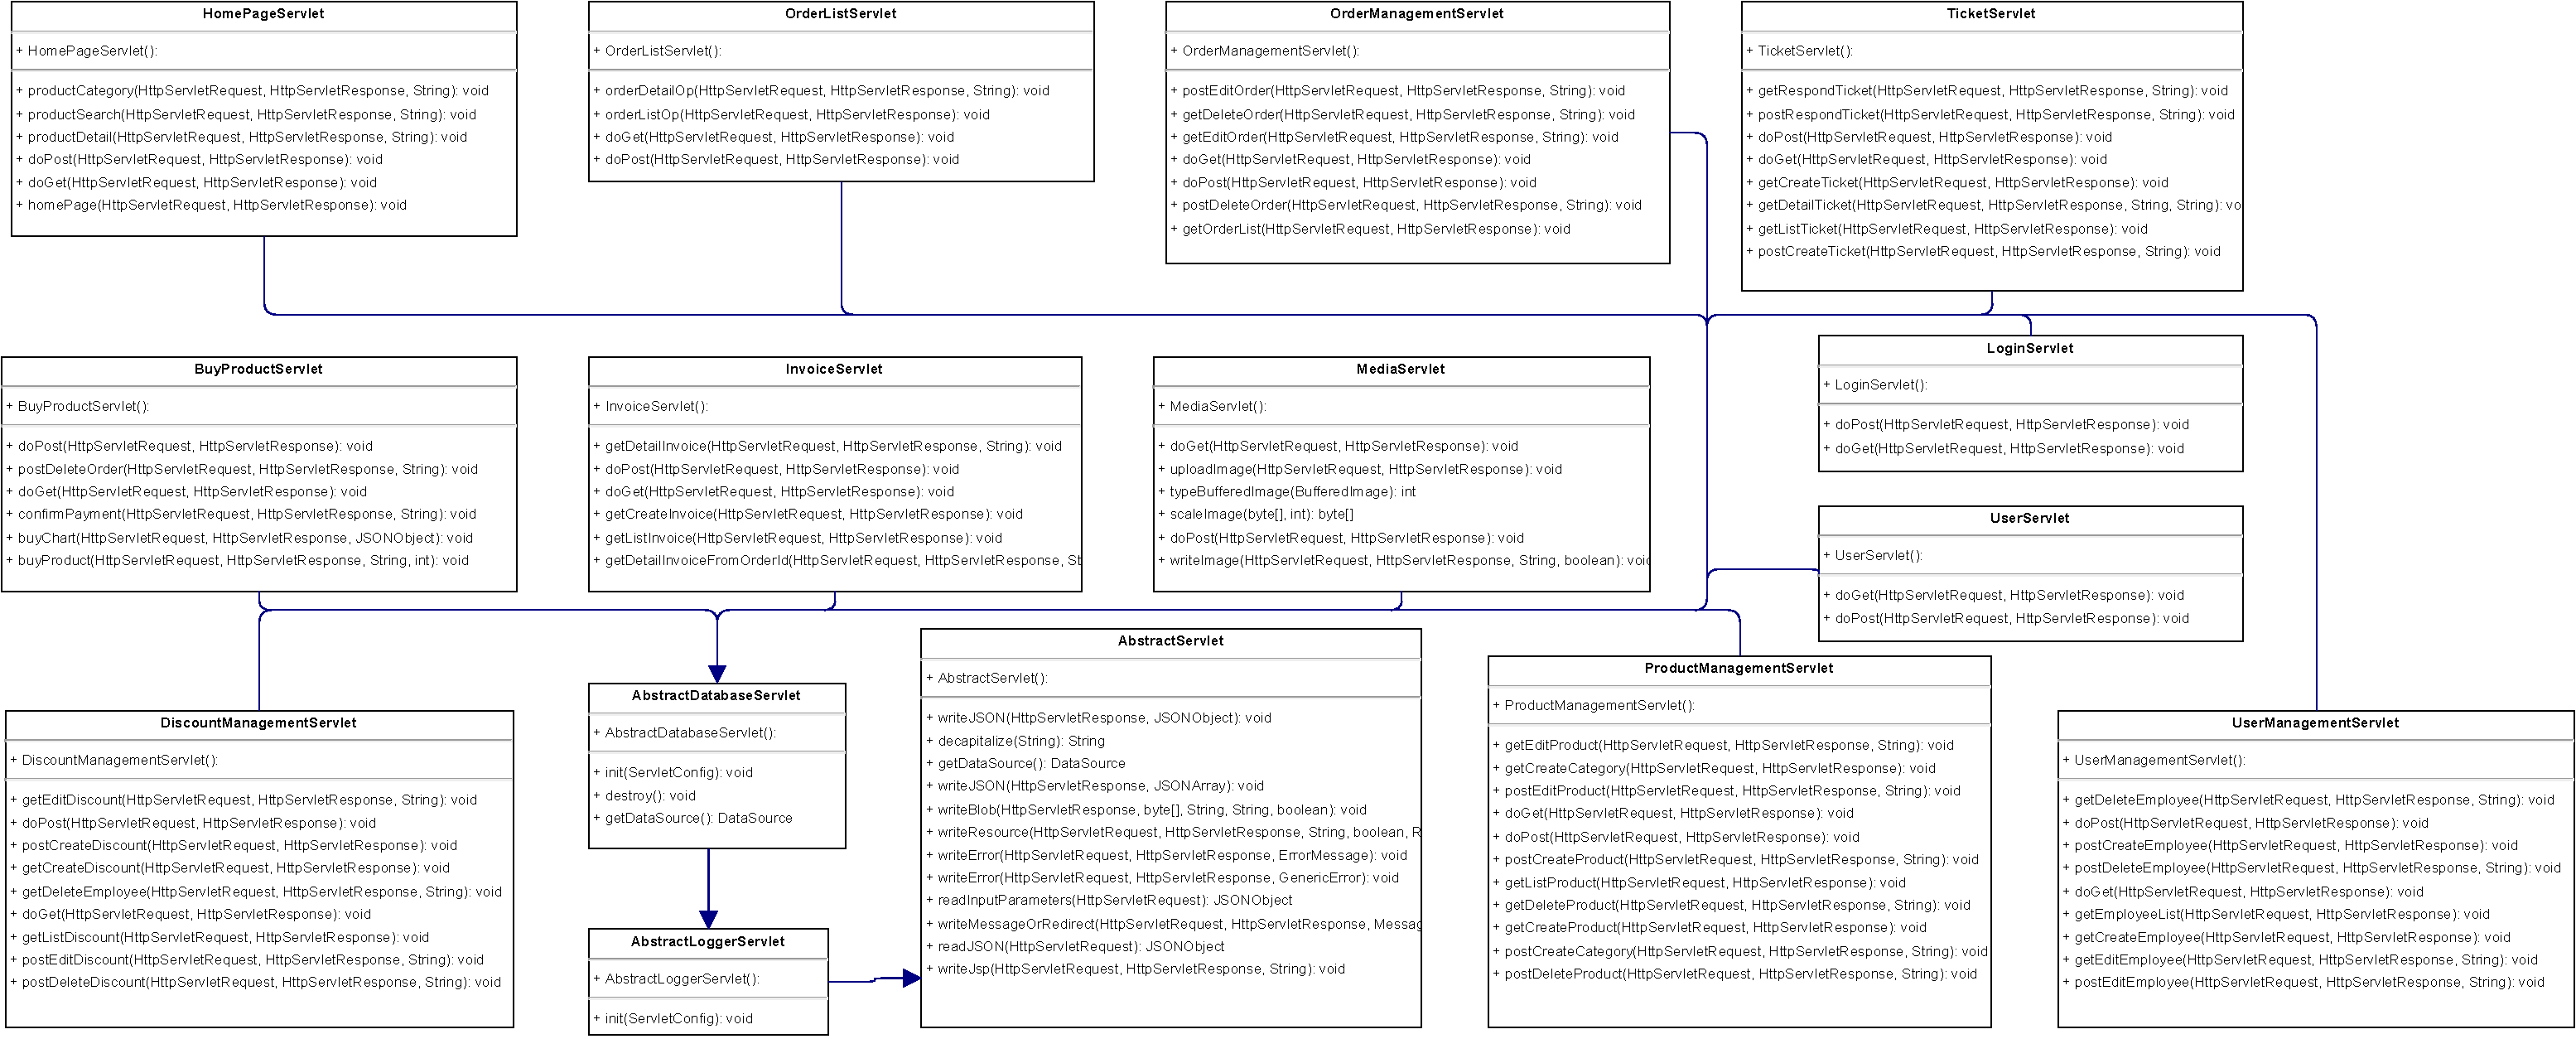
\includegraphics[width=\textwidth,height=\textheight,keepaspectratio]{Schemas/servlet.drawio.pdf}
    \caption{Servlet class diagram}
    \label{fig:ServletClassDiagram}
\end{figure}

\subsection*{Filter}

    
The filter package contains an abstract class that takes care of 
initializing the common filter information. The 4 filter classes that 
extend the abstract one, take care of filtering the data in the session.

In the figure \ref{fig:FilterClassDiagram} you can see the architecture 
of the filters. In the next pages we will use
the first letter of the filter class name to indicate the filter.
In particular \textbf{L} for \texttt{LoginFilter}, 
\textbf{A} for \texttt{AdminFilter}, \textbf{E} for 
\texttt{EmployeeFilter} and \textbf{C} for \texttt{CustomerFilter}.

A brief description of what the filters do:
\begin{itemize}
    \item \texttt{LoginFilter} checks if the user is logged in
    \item \texttt{CustomerFilter} checks if a customer is logged in
    \item \texttt{EmployeeFilter} checks if an employee is logged in
    \item \texttt{AdminFilter} checks if an administrator is logged in
\end{itemize}

\begin{figure}[H]
    \centering
    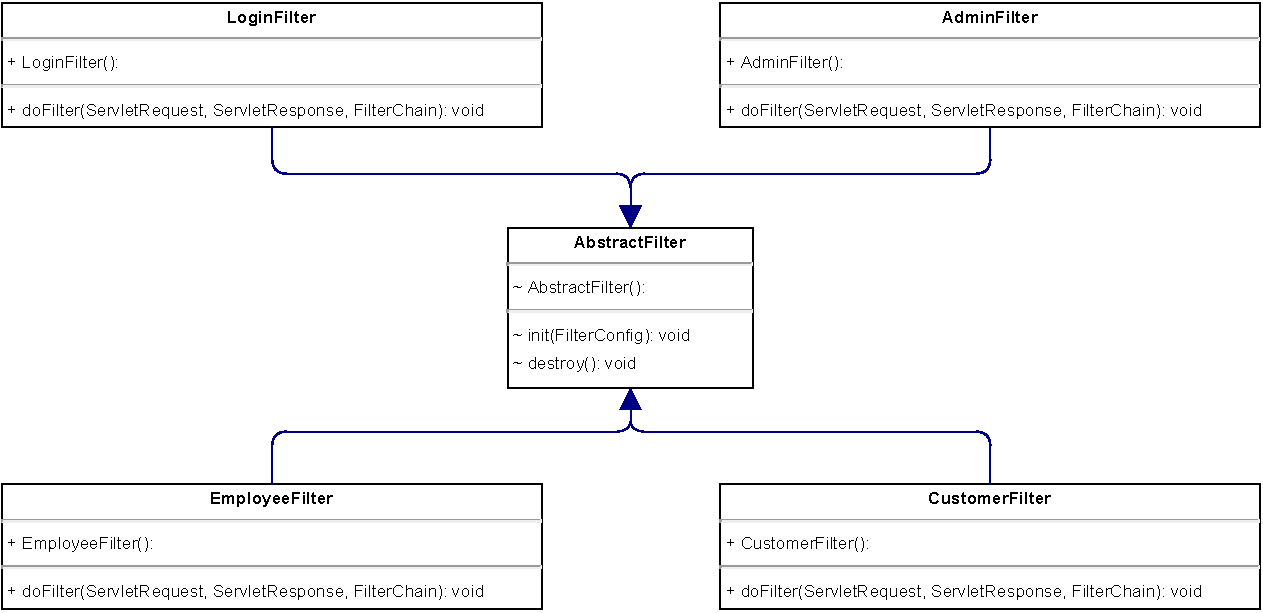
\includegraphics[width=0.7\textwidth]{Schemas/filter.drawio.pdf}
    \caption{Filter class diagram}
    \label{fig:FilterClassDiagram}
\end{figure}